\documentclass[11pt]{utalcaDoc}
\usepackage{alltt}
\usepackage{underscore}
\usepackage[utf8]{inputenc}
\usepackage[activeacute,spanish]{babel}
\usepackage{verbatim}
\usepackage[pdftex]{graphicx}
\usepackage{ae}
\usepackage{amsmath}
\usepackage{amsfonts}
\usepackage{pdflscape}
\usepackage{inconsolata}
\usepackage{url}
\usepackage{hyperref}
\usepackage{listings}
% \usepackage{placeins}
\usepackage[section]{placeins}
\usepackage[stable]{footmisc}
\usepackage{minted}
\usepackage{multicol}

\usepackage{csquotes}
\title{{\bf Seguridad Informática}\\ Laboratorio 5}
\author{Erik Regla\\ eregla09@alumnos.utalca.cl}
\date{\today}

\begin{document}
\maketitle
\newpage
\tableofcontents
\newpage

\section{Actividades}
Para esta actividad deberá crearse una cuenta en el portal Hack The Box
(https://www.hackthebox.eu/).

\subsection[Desarrollo]{Desarrollo}



\begin{figure}[H]
	\centering
	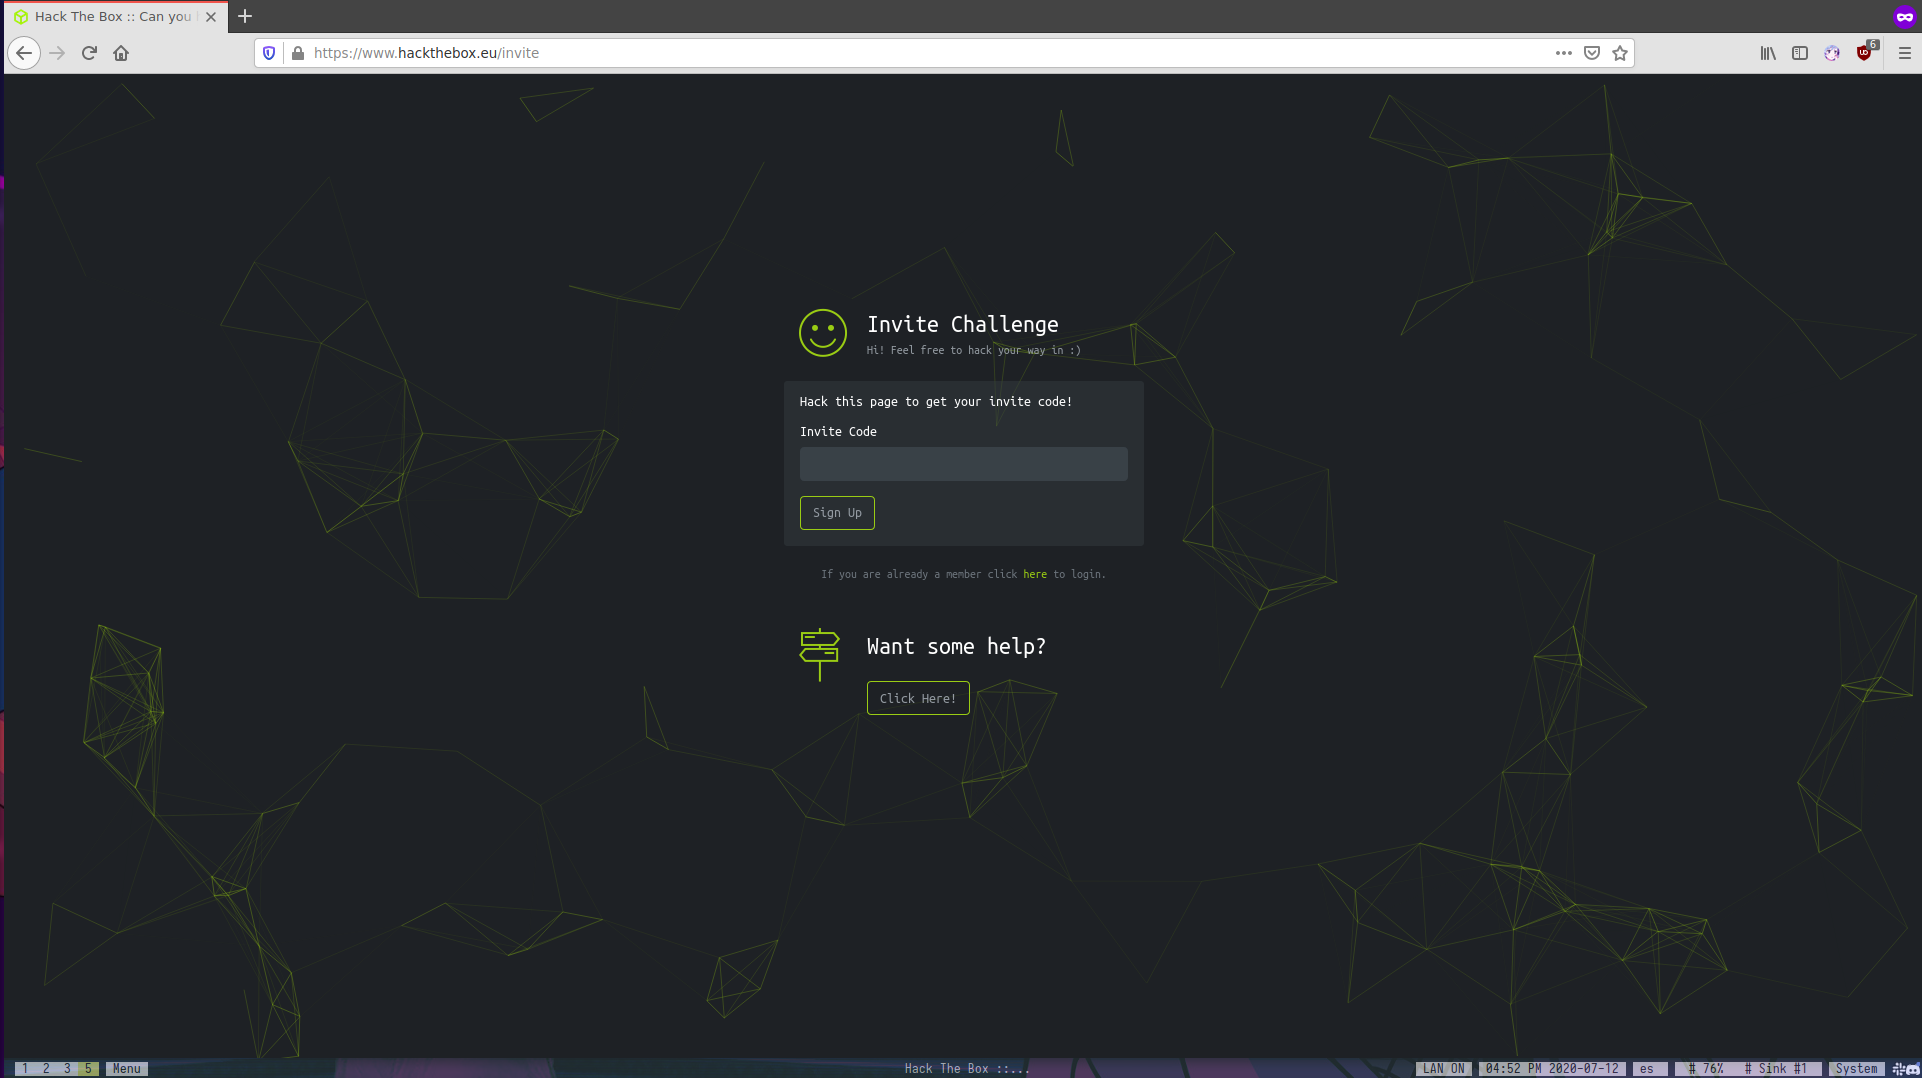
\includegraphics[width=.9\textwidth]{images/01.png}
	\caption{Al ingresar para crear la cuenta, se solicita utilizar un código de invitación, sin embargo no se explicita de donde este ses obtenido.}
\end{figure}
\begin{figure}[H]
	\centering
	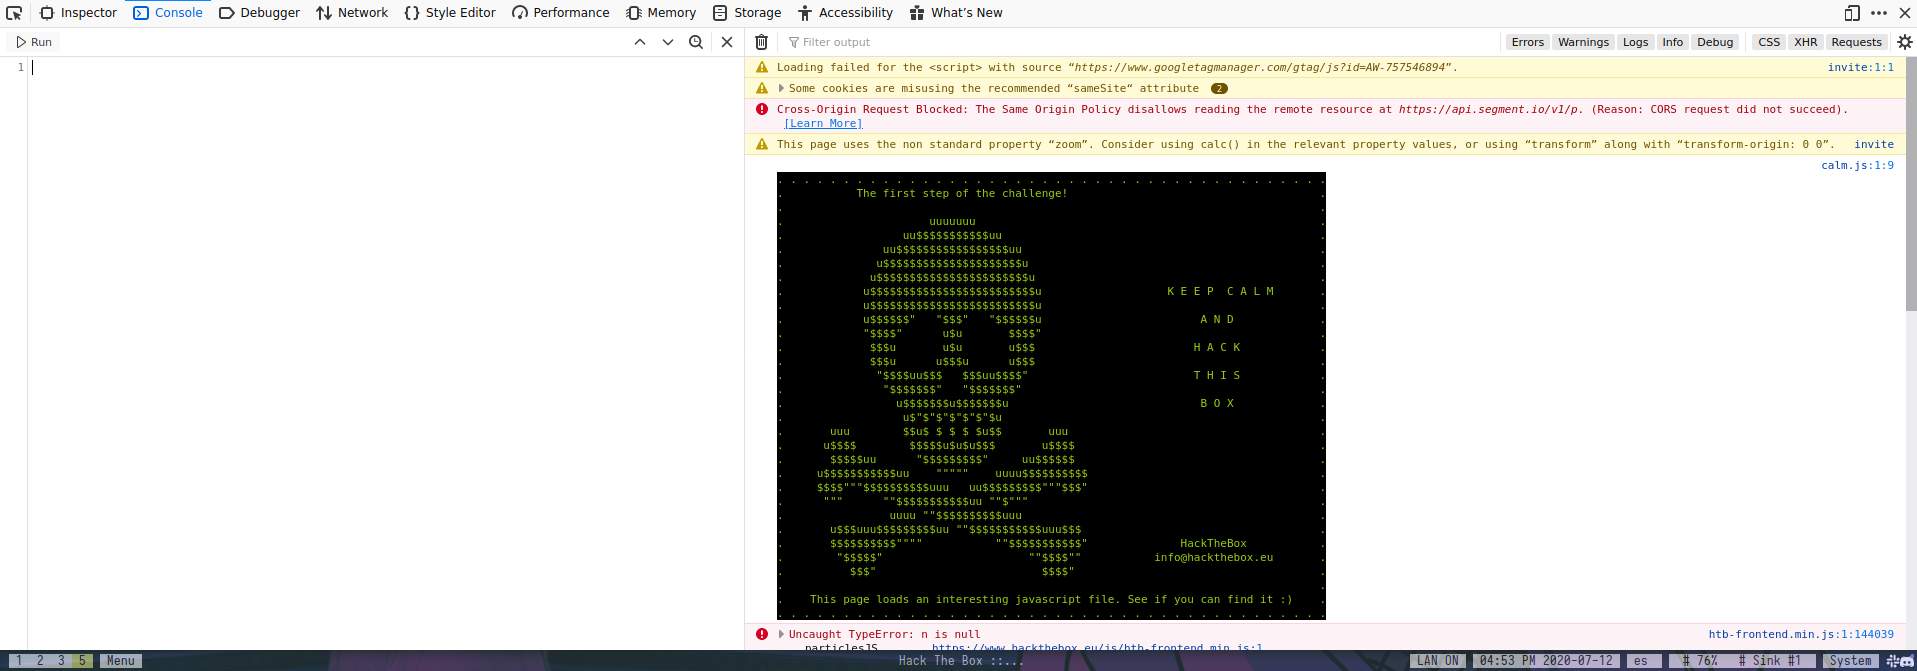
\includegraphics[width=.9\textwidth]{images/02.png}
	\caption{El primer intento consiste en ver si la consola entrega alguna información interesante. Sin embargo, somos bienvenidos con un mensaje de buscar algun archivo interesante dentro de los scripts descargados.}
\end{figure}
\begin{figure}[H]
	\centering
	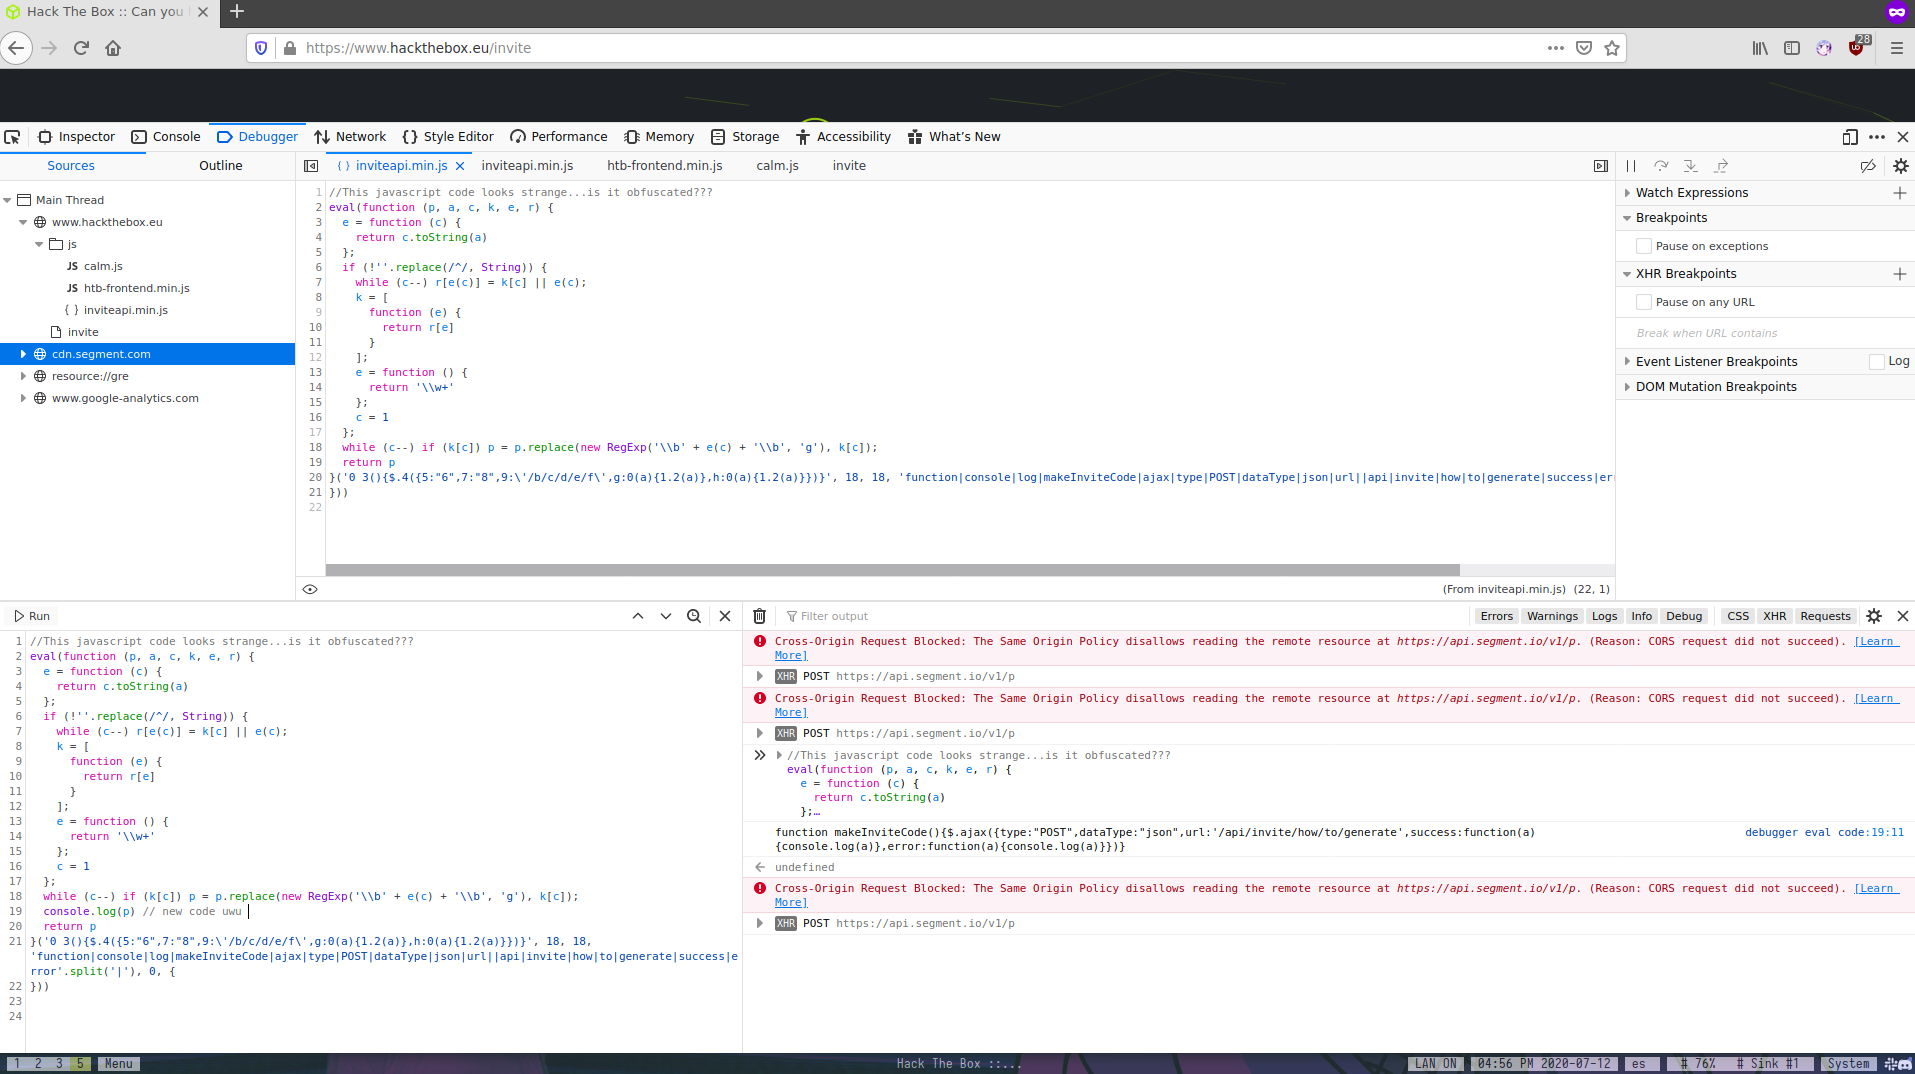
\includegraphics[width=.9\textwidth]{images/03.png}
	\caption{ El archivo encontrado (extremadamente obvio por cierto) pertenece a un código obfuscado. Ahora, esta ejecución per-se no es real. Cuando un código es obfuscado para luego ser ejecutado suele tener un proceso de carga en etapas posteriores, sin embargo este código nunca es ejecutado. Por tanto procedemos a ejecutar el código y ver su salida (aunque normalmente esto no se hace ya que si no sabes con seguridad que hace, es posible que estés cayendo en un honeypot si no tienes el entorno aislado). }
\end{figure}
\begin{figure}[H]
	\centering
	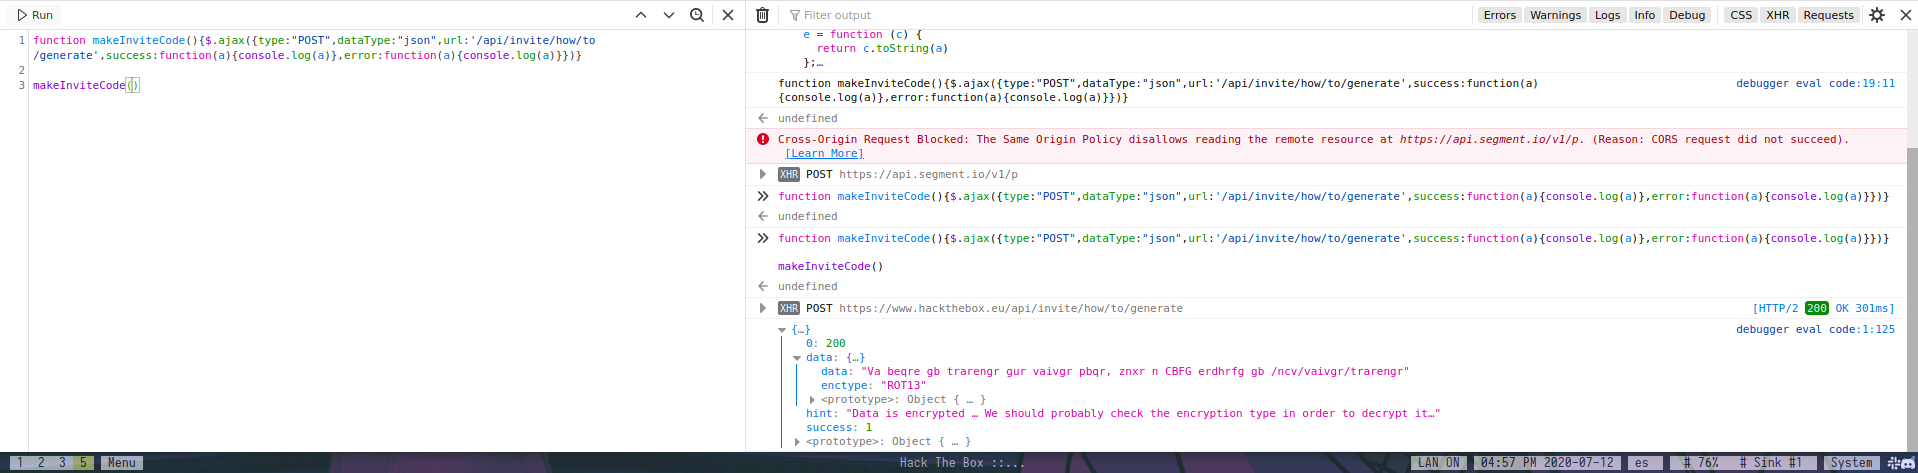
\includegraphics[width=.9\textwidth]{images/04.png}
	\caption{ El resultado de el código obfuscado es una llamada a la api del sitio, la cual devuelve un contenido encriptado (oh si, súper encriptado), el cual indica claramente que es ROT13. }
\end{figure}
\begin{figure}[H]
	\centering
	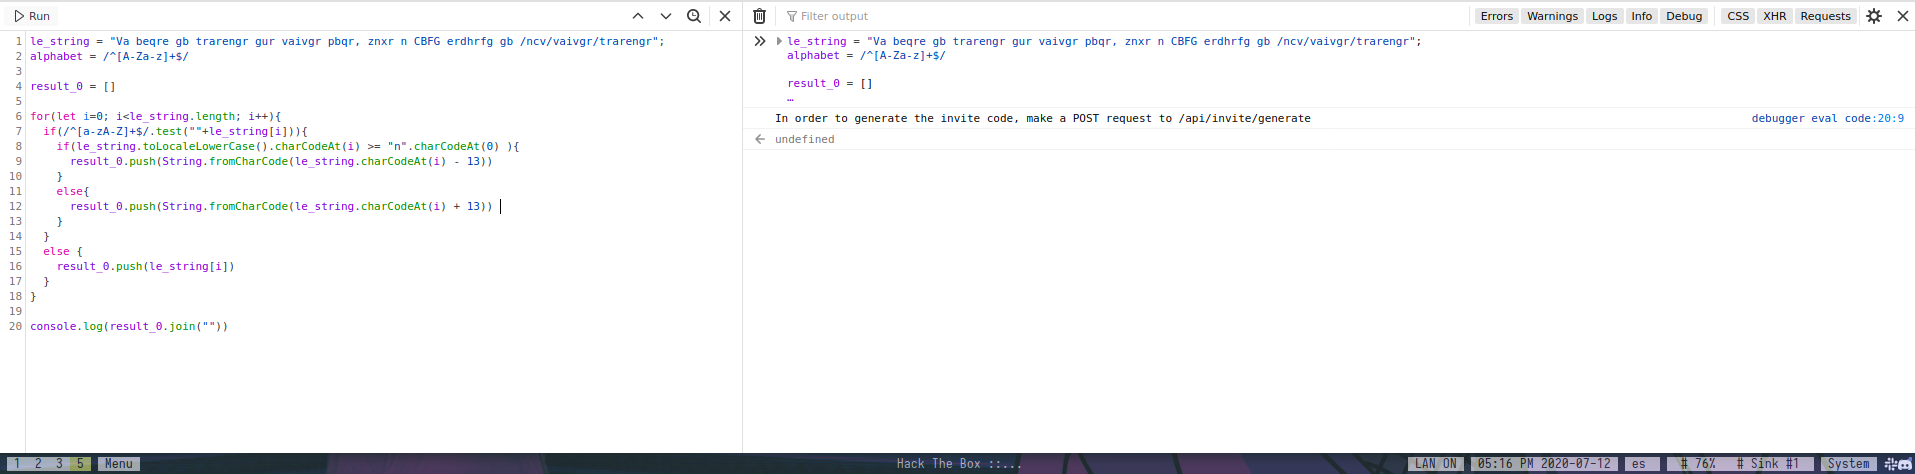
\includegraphics[width=.9\textwidth]{images/05.png}
	\caption{ Al revertir ROT13 tenemos un mensaje donde nos dicen que tenemos que ejecutar una llamada POST a otra dirección para tener nuestro invite-code. }
\end{figure}
\begin{figure}[H]
	\centering
	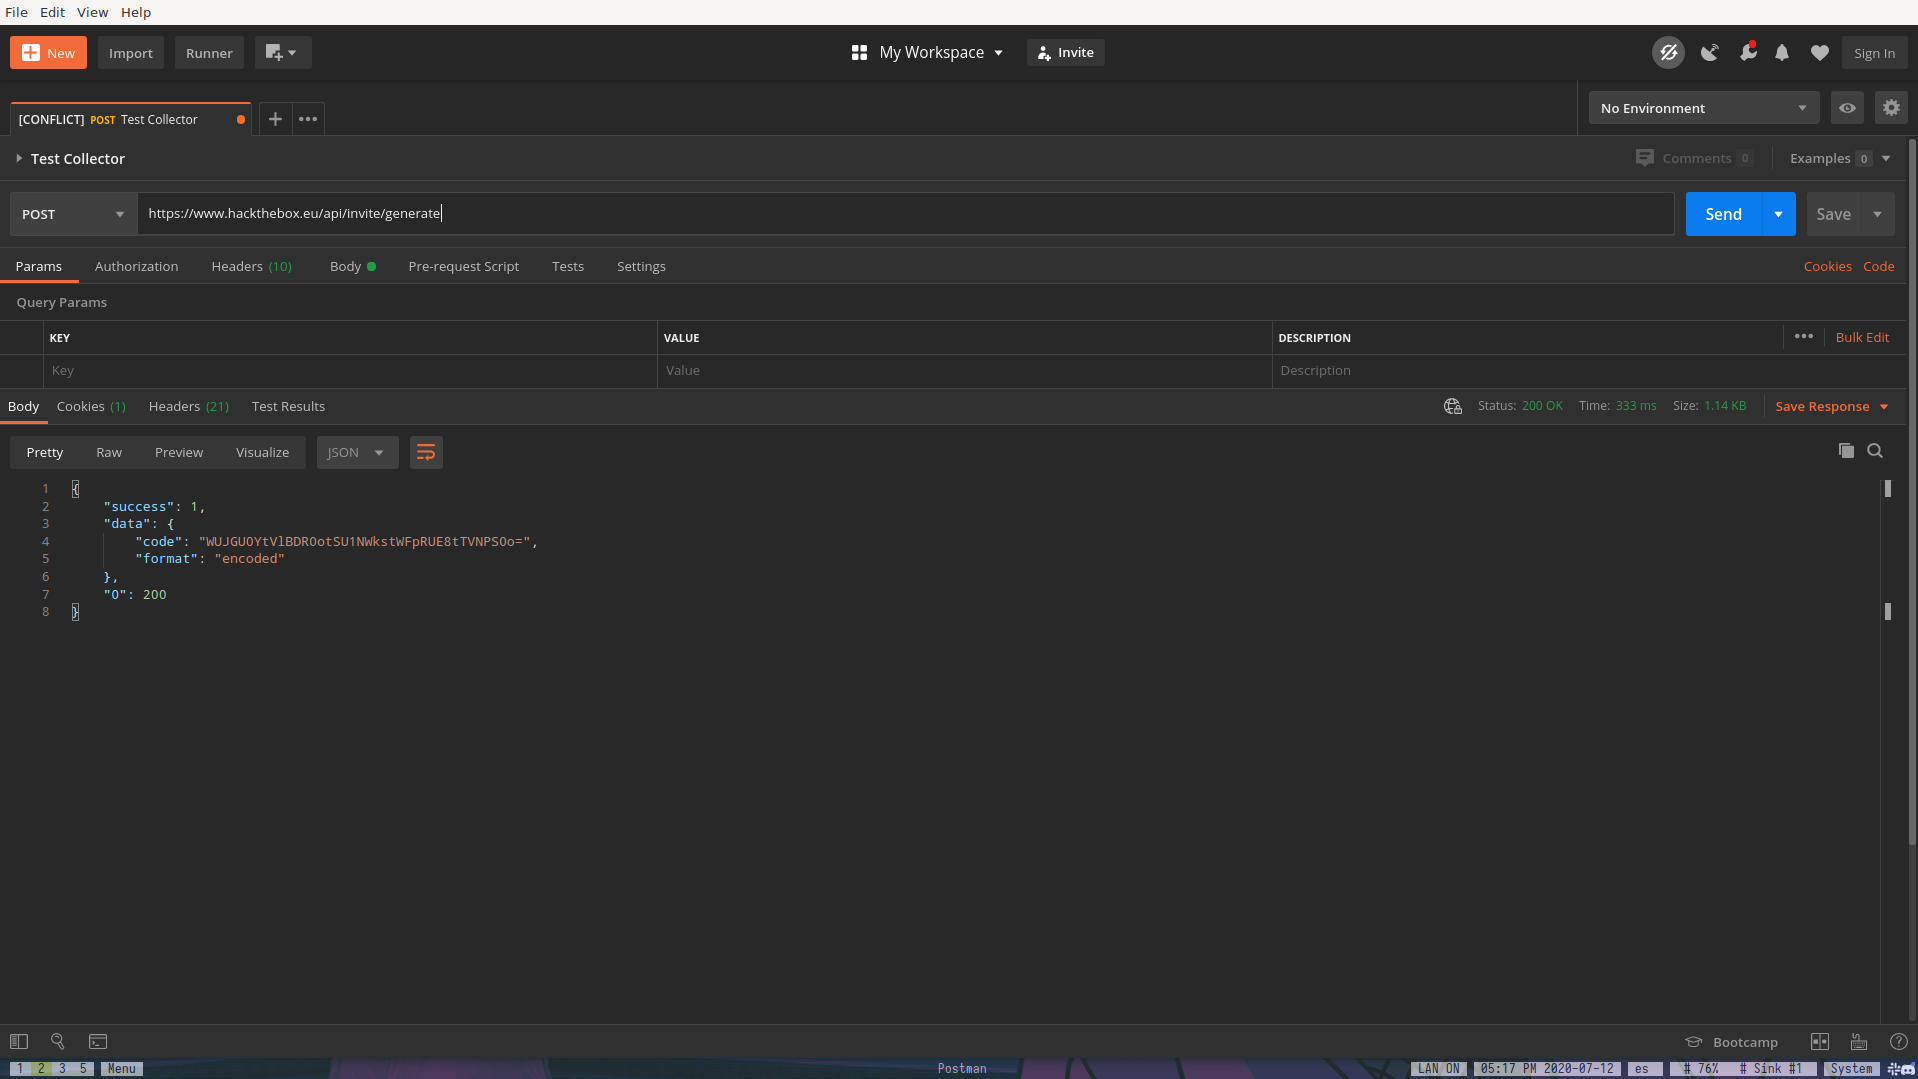
\includegraphics[width=.9\textwidth]{images/06.png}
	\caption{ Ejecutamos la llamada pero resulta que el resultado viene codificado como base64 (delatado por la parte final).}
\end{figure}

\begin{figure}[H]
	\centering
	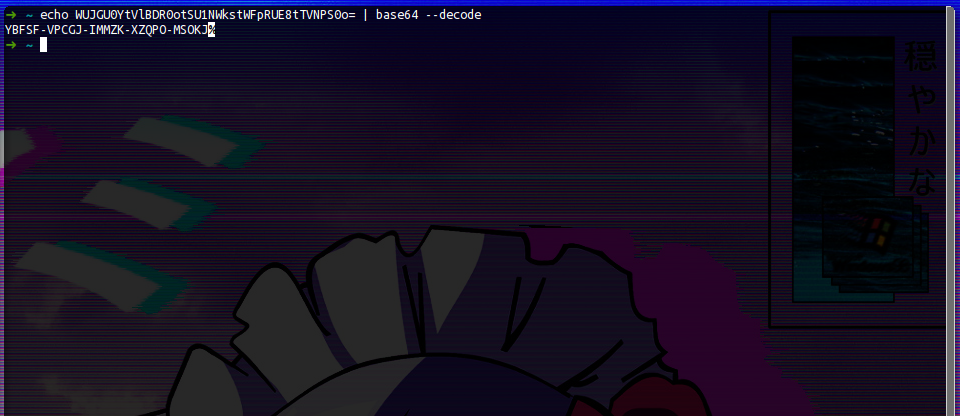
\includegraphics[width=.9\textwidth]{images/07.png}
	\caption{ Revertimos el codificado y tenemos algo que parece... Un invite code -aunque en realidad mas parece una serial de Windows XP -. }
\end{figure}

\begin{figure}[H]
	\centering
	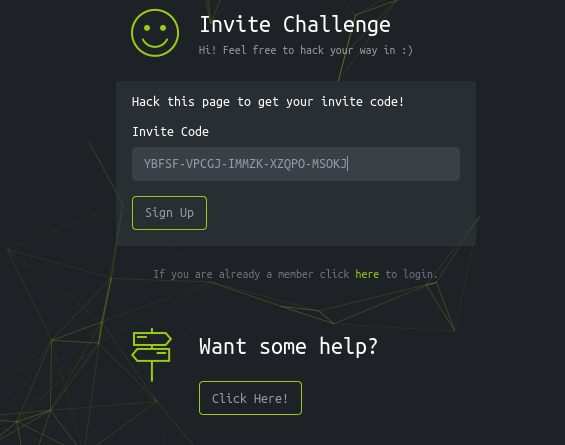
\includegraphics[width=.9\textwidth]{images/08.png}
	\caption{ Pegamos el invite code... }
\end{figure}

\begin{figure}[H]
	\centering
	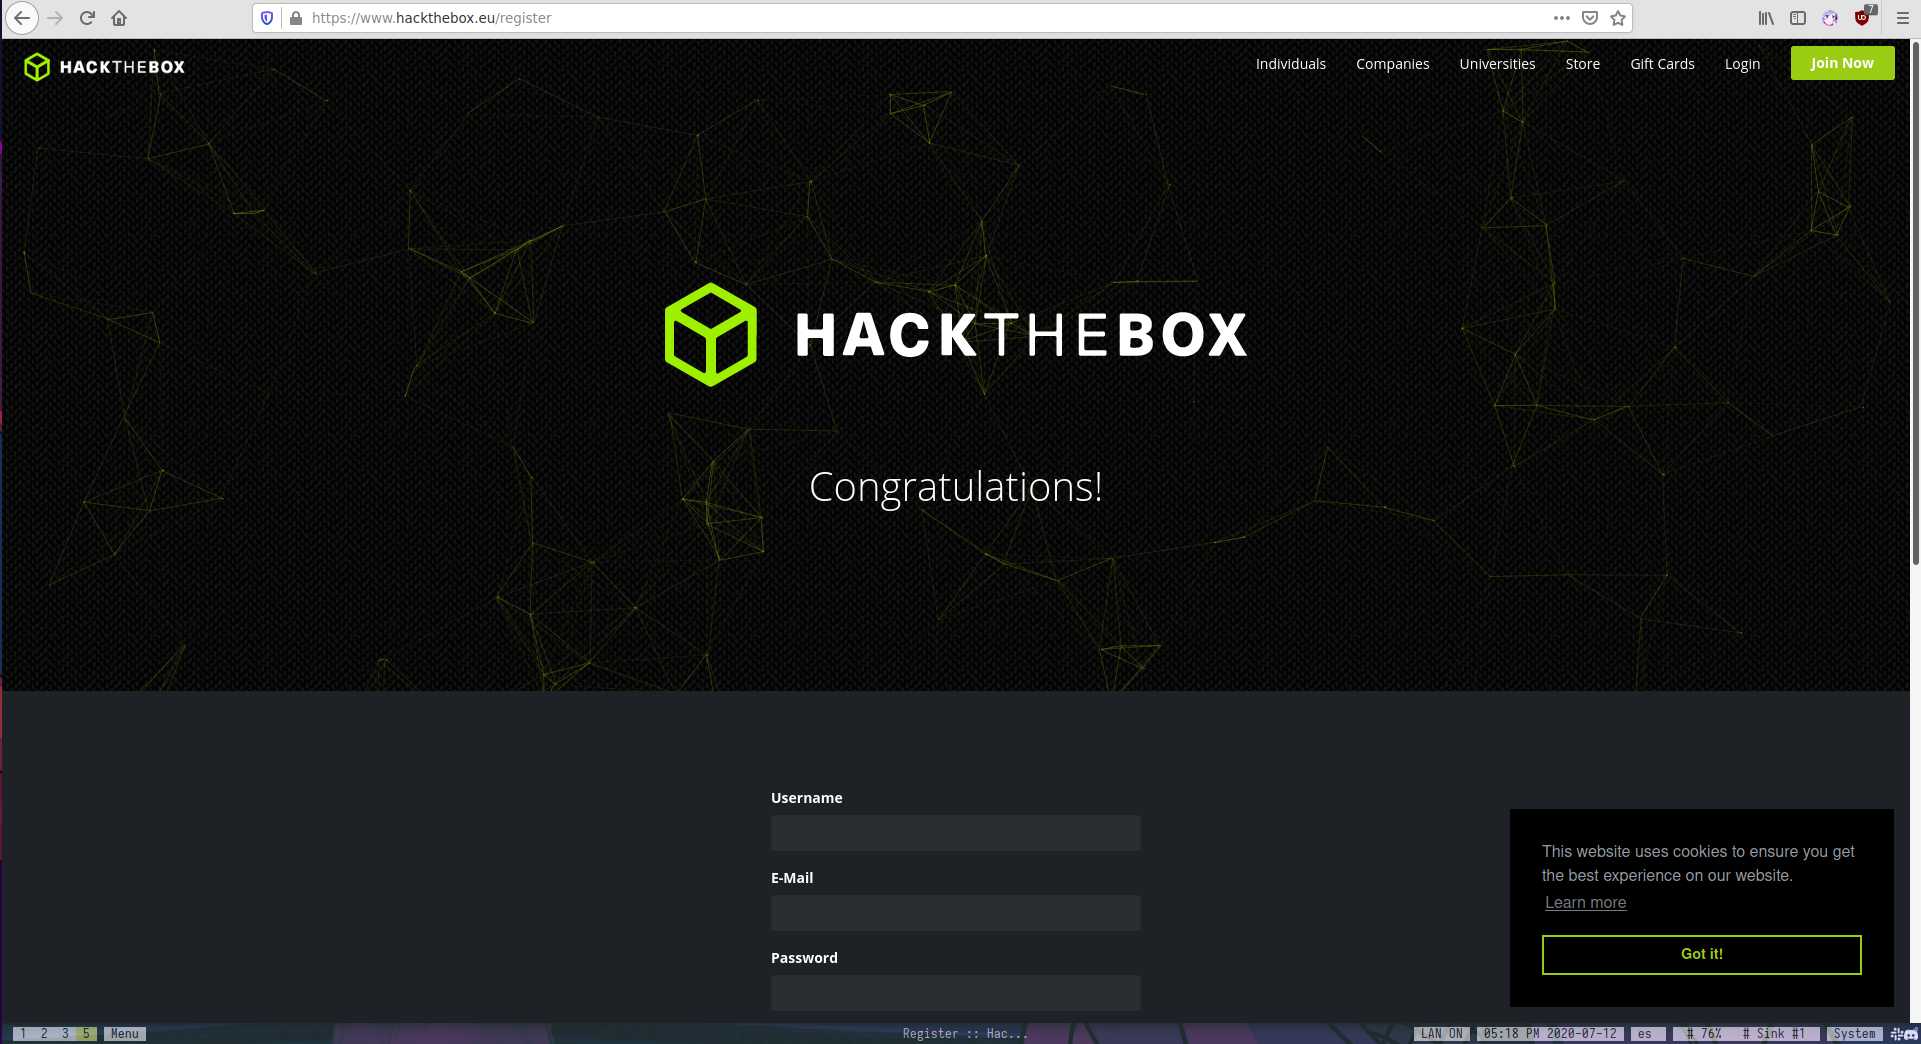
\includegraphics[width=.9\textwidth]{images/09.png}
	\caption{ Y listo, fuimos aceptados para poder generar nuestra cuenta. }
\end{figure}

\begin{figure}[H]
	\centering
	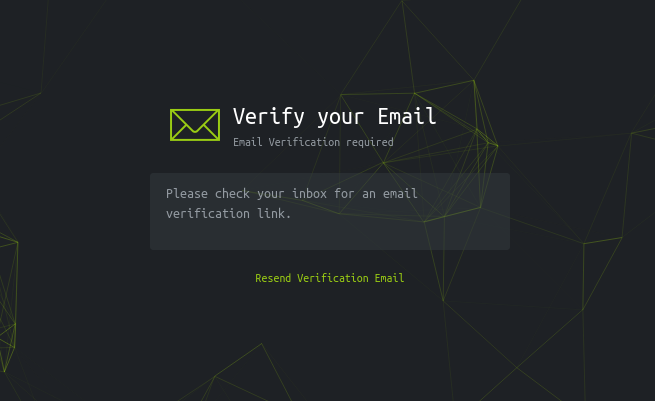
\includegraphics[width=.9\textwidth]{images/10.png}
	\caption{ Revisamos el correo de confirmación... }
\end{figure}

\begin{figure}[H]
	\centering
	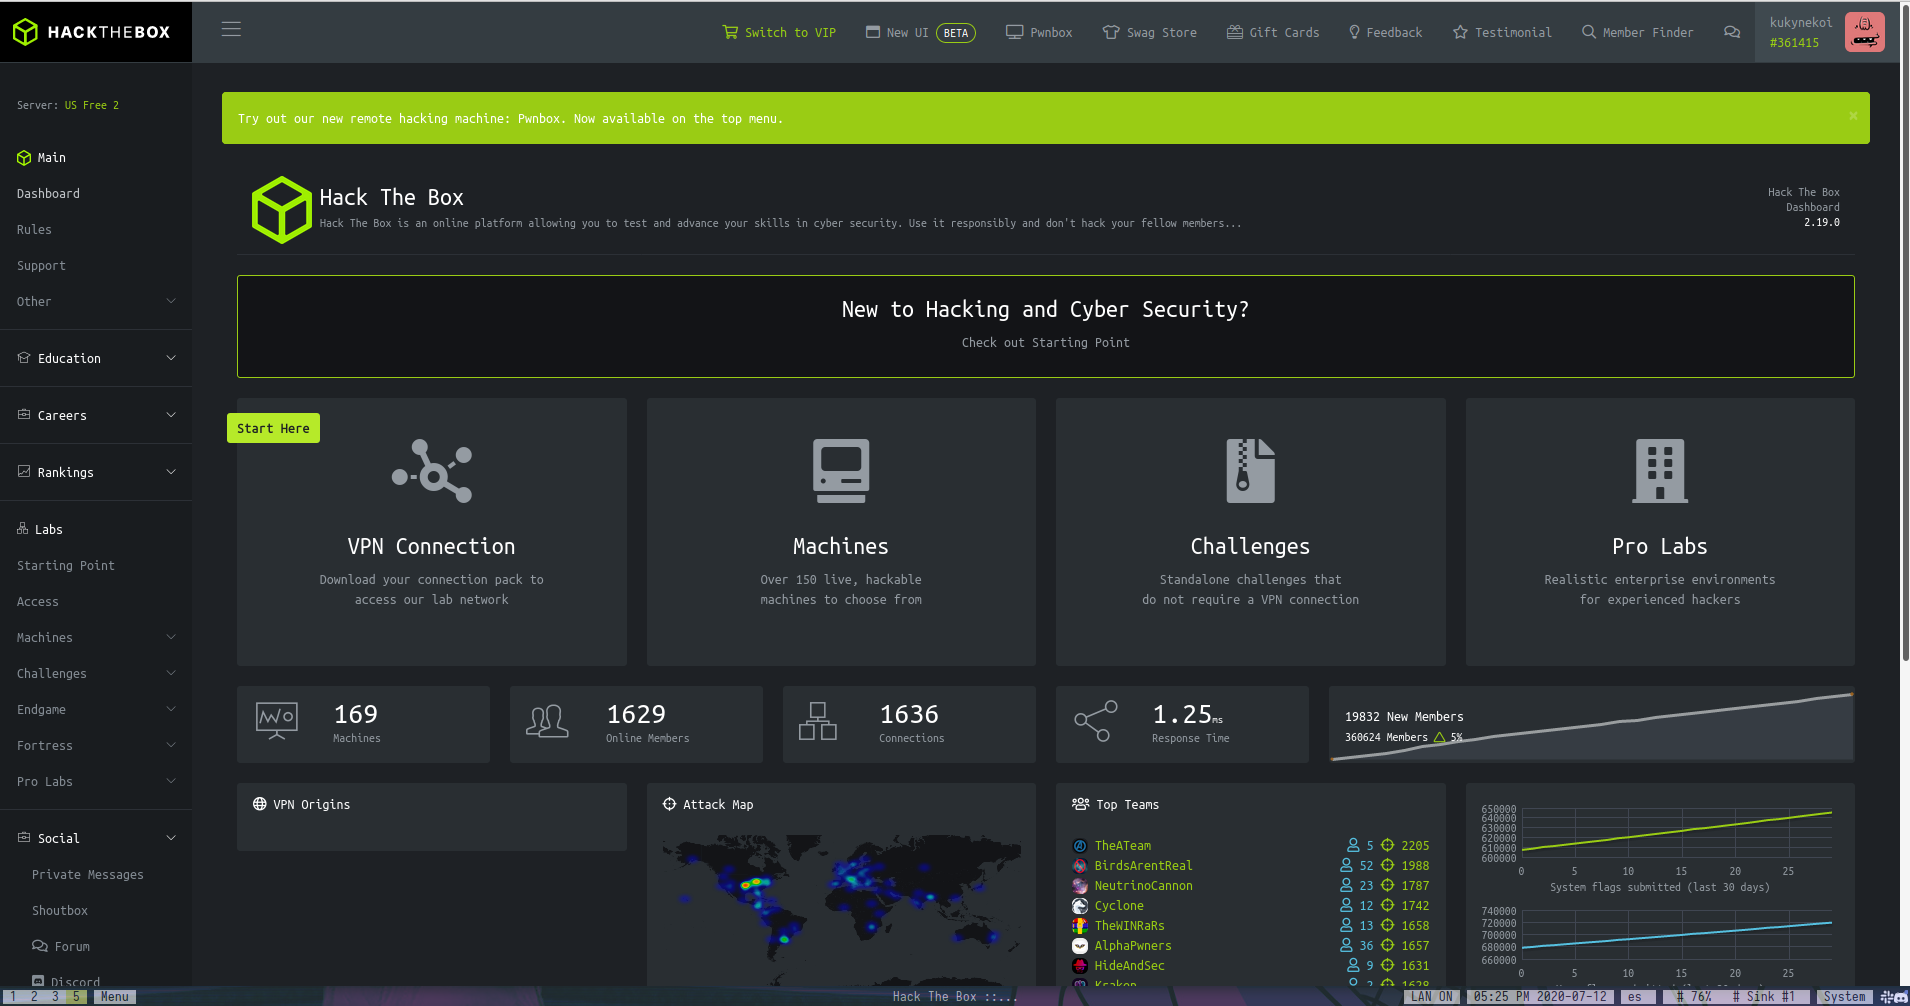
\includegraphics[width=.9\textwidth]{images/11.png}
	\caption{ Y listo, logramos registrar nuestra cuenta en el sitio. }
\end{figure}



\begin{thebibliography}{9}
	\bibitem{REF:self}
	Mi repositorio
	\textit{GitHub Repository}.
	https://github.com/KukyNekoi/UTAL/tree/master/ComputerScience
\end{thebibliography}

\end{document}